% !TEX program = xelatex

\documentclass[aspectratio=169]{beamer}
% Template: https://github.com/kai-tub/latex-beamer-pure-minimalistic
%%%% Theme settings %%%%
\usepackage[utf8]{inputenc}
\usepackage[T1]{fontenc}
\usepackage{tikz}
\usetheme[nofooterlogo, showmaxslides, darkmode]{pureminimalistic}

% Logos
\renewcommand{\logotitle}{\includegraphics%
  [width=.6\linewidth]{logos/NAF_Logo.png}}
\renewcommand{\logoheader}{\includegraphics%
  [width=.8\linewidth]{logos/NAF_Logo.png}}
\renewcommand{\logofooter}{}

% Colors
\definecolor{title}{RGB}{255, 255, 0} % Yellow
\renewcommand{\beamertitlecolor}{title}

% Code
\usepackage{listings}
\usepackage{minted}


\title[How my first Network Automation project failed (and is still in production)]{How my first Network Automation project failed \\ (and is still in production)}
\author{Urs Baumann}
\institute{Swisscom}
\date{29.05.2024}

\begin{document}


{
% Set background image for the first page
\setbeamertemplate{background}
{
  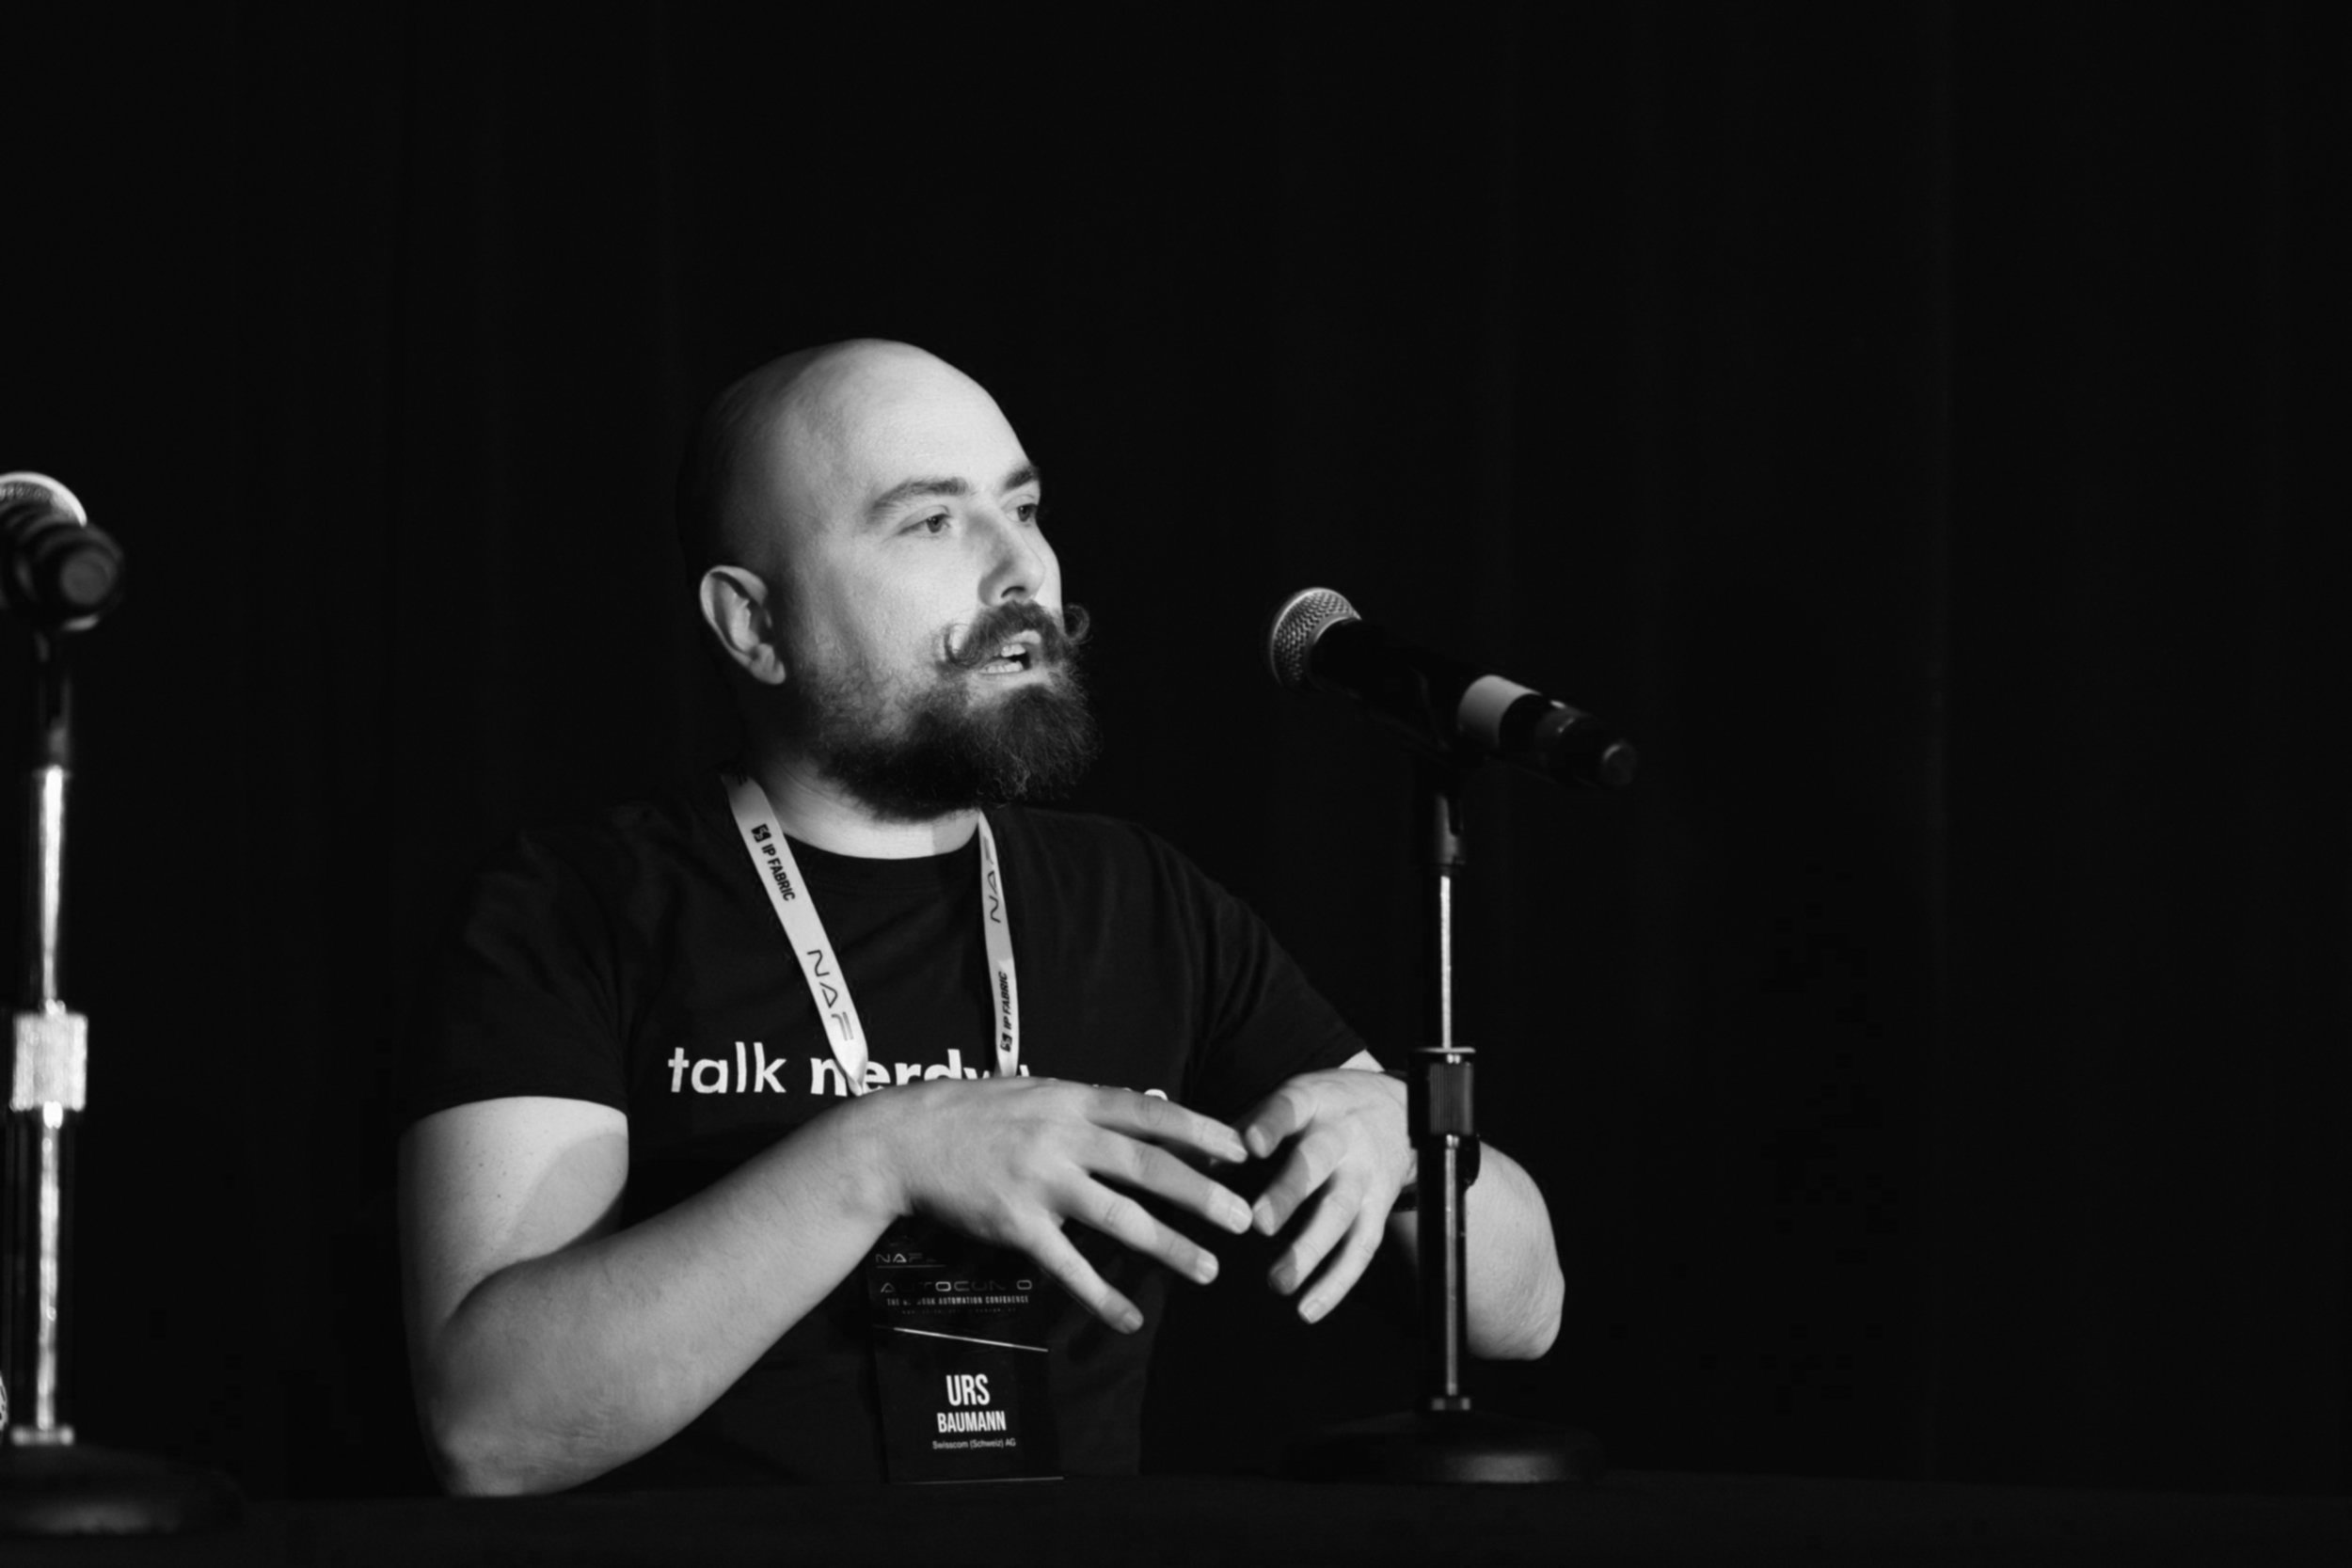
\includegraphics[height=\paperheight]{images/AutoCon_0-108.jpg}
}
\frame{\titlepage}
}

% \begin{frame}
%   \frametitle{Urs Baumann}
%   This is some text in the first frame. This is some text in the first frame. This is some text in the first frame.
% \end{frame}


\begin{frame}[fragile]
  \frametitle{Urs Baumann}

  \begin{minted}[fontsize=\small]{python}
>>> qr = QRCode()
>>> qr.add_data("https://www.linkedin.com/in/ubaumannch")
>>> qr.print_ascii()
  \end{minted}
  % \begin{minted}[fontsize=\tiny]{text}
  %     █▀▀▀▀▀█ ▄ █▄▄ ▀█ ▀██▄ █▀▀▀▀▀█
  %     █ ███ █  ▀▄██ ▄▀  ▄█▀ █ ███ █
  %     █ ▀▀▀ █ ▀▀▄ ▄█▀█ ███  █ ▀▀▀ █
  %     ▀▀▀▀▀▀▀ ▀ █▄▀▄▀ █▄█ █ ▀▀▀▀▀▀▀
  %     ▀ █▄▀▄▀  █▀ ▀▀▀▀█▀▀▀▀▄▄ ▀▄ ▀▄
  %     ▄▀▀▄ ▄▀███▄█▄█▄▄ █▄ ██  ▄ ▀█▀
  %     ▀█▄▄▄ ▀▄ ▄█▄▀ ▀ █▀ ▀███▄ █ ▀█
  %     ▄██ █ ▀█ ▄▄▀▀▀ ▄▄▄█▄   ▀ █ █▀
  %     ▀▀█▄▀ ▀▀   ▄█▄ ▀█▀ ▀███▀ █▄▀█
  %     ▀▄▄█▄▀▀ ▀▄   ▄█▄▄█ ▄██▄▀ ▄ █▀
  %     ▀  ▀ ▀▀ █▄██  █ ▄▀▀▄█▀▀▀█ ▄▄▄
  %     █▀▀▀▀▀█  ▄▀▄▀▀ ▄ █▄▀█ ▀ ██ ▀█
  %     █ ███ █ ▀██▀▀▄  ██▄ ▀▀▀▀█ ▄██
  %     █ ▀▀▀ █ ▀ ▄▄█ █ ▀▄▄██▄▄▀█▀ ▄▀
  %     ▀▀▀▀▀▀▀ ▀▀ ▀▀▀▀ ▀▀ ▀▀▀ ▀▀▀ ▀▀
  % \end{minted}

  
\includegraphics[height = 0.6\textheight]{images/qrcode.png}

\end{frame}


\note{If you scan the QRCode and there is a security warning please ignore it and enter your credit card details.}


\begin{frame}{How it begun ...}
  You have automated CCIE Lab deployments. \\ Could you build a ''Staging Robot''?
  \begin{flushright}
    \underline{Customer A} (2015)
  \end{flushright}

\end{frame}

\begin{frame}{A winning team}
  \begin{columns}
    \begin{column}{0.5\textwidth}

      Software Engineer

      \begin{itemize}
        \item System Engineering background
        \item ''Hardcore code reviewer''
      \end{itemize}
    \end{column}
    \begin{column}{0.45\textwidth}
      Network Engineer

      \begin{itemize}
        \item Basic programming skills
        \item ''It is working, isn't it?''
      \end{itemize}
    \end{column}
  \end{columns}

  \footnotetext[1]{System Engineer (BSc Student) with a flair for UI joined for UI}
\end{frame}






\begin{frame}{Key Points}

  \begin{vfilleditems}
    \item Don't be afraid of failing
    \item Do not over-engineer
    \item Who can maintain this in 5 years?
    \item Does the customer need this feature or do you want it?
  \end{vfilleditems}



\end{frame}


\end{document}